

\Oznaka{}{}{LaTeX}
\Rokovi{2018-L4,2023-L4}
%\noindent 
%\textbf{\stepcounter{zadatak}
%\thecjelina.\thezadatak.}
\Tekst{
Vanjska sila iznosa $\vec{F_0}=18\ N$ djeluje pod kutom od $\alpha=28 ^\circ$ prema horizontali na blok mase $m=3\ kg$. Izračunajte iznos 
ubrzanja kada je kinetičko trenje između bloka i podloge $\mu_k=0,4$.

\begin{figure}[h]%{r}{0.4\textwidth} % Inline image example
  \begin{center}
    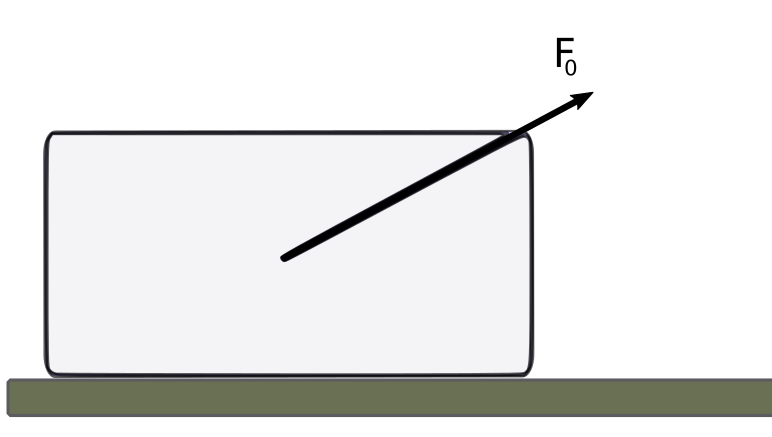
\includegraphics[scale=0.29]{../03_Dinamika_materijalne_tocke/Zadatak_D201.png}
  \end{center}
  %\caption{Fish}
\end{figure}

}
\Rjesenje{$\vec{a}=2,5\ ms^{-2} $}
\Postupak{

$$ \vec{F}_R=\sum_i \vec{F}_i=m\vec{a}$$
$$\vec{F}_0+\vec{G}+\vec{R}+\vec{F}_{tr}=m\vec{a} $$
Radimo projekcije na $y$ i $z$ os
$$ \textbf{y:}\ \ \vec{F}_0\cdot\vec{j}+\vec{G}\cdot\vec{j}+\vec{R}\cdot\vec{j} + \vec{F}_{tr}\cdot\vec{j}= m\vec{a}\cdot\vec{j}\ \ \ \ \  /\cdot\vec{j} $$
$$ |\vec{F}_0||\vec{j}|\cos\alpha  + |\vec{G}||\vec{j}|\cos \frac{\pi}{2}  +  |\vec{R}||\vec{j}|\cos \frac{\pi}{2} +  |\vec{F}_{tr}||\vec{j}|\cos\pi
= m|\vec{a}||\vec{j}|\cos0 $$
\begin{equation}
 F_0\cos\alpha+ 0 +0 -F_{tr}=ma 
 \label{zadata_4_1_1}
\end{equation}
 


$$  \textbf{z:}\ \ \vec{F}_0\cdot\vec{k} +  \vec{G}\cdot\vec{k}  + \vec{R}\cdot\vec{k} + \vec{F}_{tr}\cdot\vec{k} = m \vec{a}\cdot\vec{k} \ \ \ \ \  /\cdot\vec{k} $$
$$   |\vec{F}_0||\vec{k}|\cos(\frac{\pi}{2}-\alpha) +|\vec{G}||\vec{k}|\cos\pi +  |\vec{R}||\vec{k}|\cos0 + 
|\vec{F}_{tr}||\vec{k}|\cos\frac{\pi}{2}=m|\vec{a}||\vec{k}|\cos\frac{\pi}{2} $$
\begin{equation}
F_0\sin\alpha-G + R =0
\label{zadata_4_1_2}
\end{equation}
Iz gornjeg izraza možemo izraziti silu reakcije podloge
$R=mg-F_0\sin\alpha$, gdje smo za silu težu ($G$) zapisali kao masa ($m$) puta ubrzanje sile teže ($g$). 

Sila trenja koja nam se javlja u izrazu \ref{zadata_4_1_1} možemo zapisati kao umonožak 
faktura kinetičkoga trenja i sili pritiska na podlogu, a sila pritiska na podlugu je jednaka težini tijela koja je po iznosu jednaka sili reakcije 
podloge tako pišemo:
$F_{tr}=\mu_k F_{\bot}=\mu_k T=\mu_k R$. 
Silu reakcije podloge možemo zamjeniti izrazom koji smo dobili iz jednadžbe \ref{zadata_4_1_2} i dobivamo konačni izraz:
$$
F_0\cos\alpha-\mu_k(mg-F_0\sin\alpha)=ma
$$
$$ a=\frac{F_0}{m}\left(\cos\alpha + \mu_k\sin\alpha\right) -\mu_k g $$

$$a = \frac{18N}{3kg}\left(\cos28^\circ + 0,4\sin28^\circ  \right) -0,4\cdot 9,81ms^{-2} =2,5\ ms^{-2} $$


}


